\documentclass[conference]{IEEEtran}
\IEEEoverridecommandlockouts
% The preceding line is only needed to identify funding in the first footnote. If that is unneeded, please comment it out.
\usepackage{cite}
\usepackage{amsmath,amssymb,amsfonts}
\usepackage{algorithmic}
\usepackage{graphicx}
\usepackage{textcomp}
\usepackage{xcolor}
\usepackage{tikz}
\usepackage{float}

\usetikzlibrary{shapes.geometric, arrows.meta, positioning, fit, backgrounds, calc}
\def\BibTeX{{\rm B\kern-.05em{\sc i\kern-.025em b}\kern-.08em
    T\kern-.1667em\lower.7ex\hbox{E}\kern-.125emX}}
\begin{document}

\title{Multi-Horizon GNSS Clock and Ephemeris Error Prediction via Stacked Ensemble Learning\\
\thanks
}

\author{\IEEEauthorblockN{1\textsuperscript{st} Anshika Shukla}
\IEEEauthorblockA{\textit{Department of Artificial Intelligence and Machine Learning} \\
\textit{CMR Institute of Technology}\\
Bengaluru, India \\
anshikashukla4@gmail.com}
\and
\IEEEauthorblockN{2\textsuperscript{nd} Manya Michelle}
\IEEEauthorblockA{\textit{Department of Artificial Intelligence and Machine Learning} \\
\textit{CMR Institute of Technology}\\
Bengaluru, India \\
12michelle004@gmail.com}
\and
\IEEEauthorblockN{3\textsuperscript{rd} Pallavi A Kumbar}
\IEEEauthorblockA{\textit{Department of Artificial Intelligence and Machine Learning} \\
\textit{CMR Institute of Technology}\\
Bengaluru, India \\
paku23csaiml@cmrit.ac.in}
\and
\IEEEauthorblockN{4\textsuperscript{th} Sharat Patil}
\IEEEauthorblockA{\textit{Department of Artificial Intelligence and Machine Learning} \\
\textit{CMR Institute of Technology}\\
Bengaluru, India \\
shpa23csaiml@cmrit.ac.in}
\and

\IEEEauthorblockN{5\textsuperscript{th} Harshavardhan Reddy A}
\IEEEauthorblockA{\textit{Department of Artificial Intelligence and Machine Learning} \\
\textit{CMR Institute of Technology}\\
Bengaluru, India \\
harshavardhan.cseaiml24le@cmrit.ac.in}
}

\maketitle

\begin{abstract}
Satellite clock errors and ephemeris inaccuracies keep GPS systems off target. Current fixes fall short — extrapolating stale corrections beyond their validity window amplifies error rapidly, whereas single-model machine learning methods fail to capture shifting patterns across multiple time scales.
This research introduces a hybrid ensemble framework where error prediction splits into three focused components: one targeting rapid variations, another managing slow drifts, while the third tracks periodic cycles. Outputs from these components are fused via linear regression, with residuals modeled using a Gaussian process, delivering calibrated uncertainty estimates alongside forecasts.
One week of real GNSS observations across multiple satellite constellations fed into the system, with forecasts generated at varying prediction horizons. It outperformed baseline approaches on both clock offset and ephemeris error prediction, with residuals conforming to Gaussian distributions — a necessary condition for reliable positioning integrity.
\end{abstract}

\begin{IEEEkeywords}
GNSS error prediction, satellite clock bias, ephemeris error, LSTM, Transformer, XGBoost, Gaussian Process, ensemble learning, uncertainty quantification
\end{IEEEkeywords}

\section{Introduction}
Satellites like GPS, GLONASS, Galileo, BeiDou, and NavIC form global networks that guide everything from farm equipment to airplane routes, along with keeping phone signals in sync. What keeps their location data reliable comes down to just two pieces sent out by each satellite: how fast its internal clock runs, alongside details about where it actually orbits. These numbers get checked now and then by stations on Earth, adjusted when needed, before being shot back up so the satellites can pass them around. Without precise updates on timekeeping and position, even small errors grow into big problems for anyone relying on the signal. Each system leans heavily on this cycle - ground teams measure, tweak, send; machines above relay what they receive.
What holds this system back most? It's the delay between updates. Clock and position data sent out reflect conditions only when measured. After that moment passes, real satellite clocks start slipping away from predicted values. Meanwhile orbits shift too - tugged by uneven gravity, sunlight pushing on surfaces, even thin air up high. These unseen nudges mean the path drawn in data slowly stops matching where the satellite actually flies. Sooner or later, what was broadcast no longer lines up with reality. That mismatch - called broadcast error - widens steadily until fresh numbers arrive. And it’s this widening gap that throws off distance estimates most in standard GNSS fixes.
Spotting and forecasting these signal mistakes matters right away for daily operations. Because a solid forecast system means better safety limits when lives are on the line - think planes landing or self-driving cars moving. It also sharpens location data by fixing outdated signals before they cause drift. On top of that, it gives ground crews clearer clues about how satellites are really performing, including early signs something might be off.
What shows up in the signal errors isn’t just noise - it shifts across different time layers, making it tough for one kind of model to handle everything. Minutes into hours, slow bends appear, shaped by clock wear and tiny unseen forces - this flow fits how recurrence-based nets track patterns over sequences[13]. Hours stretching toward a full day bring repeating shapes tied to orbit angles, like when a satellite sees the same sun-Earth layout again, along with heat swings from moving in and out of shadow - spots where tracking distant links matters most. Underlying features tie back in twisted ways to factors like how old the incoming data is, what part of the daily cycle it hits, or which type of satellite sent it - twists decision-tree hybrids untangle better than others.
Starting with insights from our analysis, one idea takes shape - a setup where different time frames get their own specialized models, later linked through a smart blending method. Instead of mixing everything at once, predictions join via a learning-based coordinator. Into this mix steps a Gaussian Process layer, adjusting leftover errors in a probability-aware way. This same piece delivers measures of doubt, something key systems need when checking reliability. What stands out in this study comes next
A split in how we handle GNSS signal errors shapes three clear parts. One piece deals with quick changes over time, using models built for sequences. Another grabs patterns that repeat far apart, handled by different specialized models. The last part uses specific traits linked to the signals, taken care of by its own model type.
One path uses LSTM plus GRU units. Another leans on attention through Transformers instead. A third builds decisions using tree splits like XGBoost does. Each runs separately at first. Predictions get saved after cross-validation folds finish. For each future step, a different Ridge model steps in. It learns how much to trust which pipeline. Weights shift based on time ahead. Final output blends these adjusted forecasts together.
A twist in the modeling approach uses a Gaussian Process on residuals, combining Matérn and periodic traits through a composite structure. This setup adjusts predictions at the end while shaping uncertainty estimates that behave more like normal distributions over time. Built into the system, these features meet strict statistical rules needed for checking GNSS signal reliability. The way uncertainties form follows patterns close to Gaussian, thanks to how the kernel blend operates behind the scenes.
Testing happened over five time spans - from 15 minutes up to a full day - using data from both mid-orbit and higher orbit satellites. Results showed cleaner error patterns than those seen in single model outputs, pointing toward more reliable predictions when combined. Each interval revealed tighter alignment with expected statistical behavior, especially at longer durations where noise usually grows. Performance held steady even as forecasting windows stretched further ahead. Patterns stayed consistent across all satellite types tested.

What comes next unfolds like this. Following that, Section II looks at past research on GNSS error models along with machine learning used for predicting time-based data. After covering those ideas, Section III walks through the method suggested here, step by step. Finally, Section IV wraps things up while pointing toward what might come later.
 

\section{Related Work}

\subsection{Classical GNSS Error Modeling}

Timing fixes sent out by navigation satellites usually take the form of a three-part math fit - covering delay, speed change, and acceleration - based on fresh measurements from Earth stations, refreshed once or twice per hour. Ground-based records later refined by the International GNSS Service deliver exact timing data every half minute, used as reference points when checking how far off the live signals might be [1]. Orbit details shared through radio include standard path shapes adjusted with periodic tweaks; for newer GPS IIF birds, that gives about 50 to 100 centimeters precision toward the center of orbit during normal operation [2]. Such older-style predictions run forward without accounting for surprises, offering fixed paths instead of error ranges or response to odd conduct.
Clock and ephemeris forecasts get a boost when Extended Kalman Filters team up with dynamic orbit techniques using physics-based motion rules [3]. Yet despite working well, they lean heavily on exact force details plus upfront info about satellite gear - making broad use tricky across different makers or models.

\subsection{Machine Learning for GNSS Error Prediction}

Machine learning's role in handling GNSS errors has drawn more interest lately. Instead of polynomials, methods like SVR and basic neural nets show better results when forecasting satellite clock drifts over brief periods [4, 5]. Temporal patterns in timing shifts catch better with LSTM [11, 12] models, some findings indicate, especially past the two-hour mark where they outperform Kalman filters [6, 7].
Lately, models built on Transformer designs started handling GNSS data sequences, using self-attention to track patterns that stretch over full orbit cycles [8]. Instead of fixed formulas, some methods turned to Gaussian Process regression - this gives not just predictions but also shows how unsure they are [9]. Yet most earlier attempts focused only on one type of forecast at a time, ignoring how errors show up across different timescales while skipping the need for normally shaped leftover errors, which safety checks require.

\subsection{Ensemble and Multi-Model Approaches}

Putting together different kinds of models often works better than relying on just one, especially in predicting patterns over time [10]. Instead of merely blending results, some approaches train another model to learn from the outputs of earlier ones - this tends to do well when those initial models think differently about the data [11]. As far as we can tell, nobody has yet built a system that uses several processing streams alongside horizon-specific learning for forecasting errors in GNSS signals. Also missing from past efforts is a method using Gaussian Processes at the final stage to meet strict normal-distribution needs tied to how these navigation systems monitor safety.

\section{Methodology}
Starting off, the suggested setup works step by step. First, crafting features leads to two separate views of the input signal. Following that, three initial models handle each view on its own. Then comes a combining stage - Ridge regression blends their results using time-range-adjusted coefficients. Afterward, leftover patterns get captured through a Gaussian Process. The full layout appears in Figure 1.

\begin{figure}[t]
\centering
\resizebox{\columnwidth}{!}{%
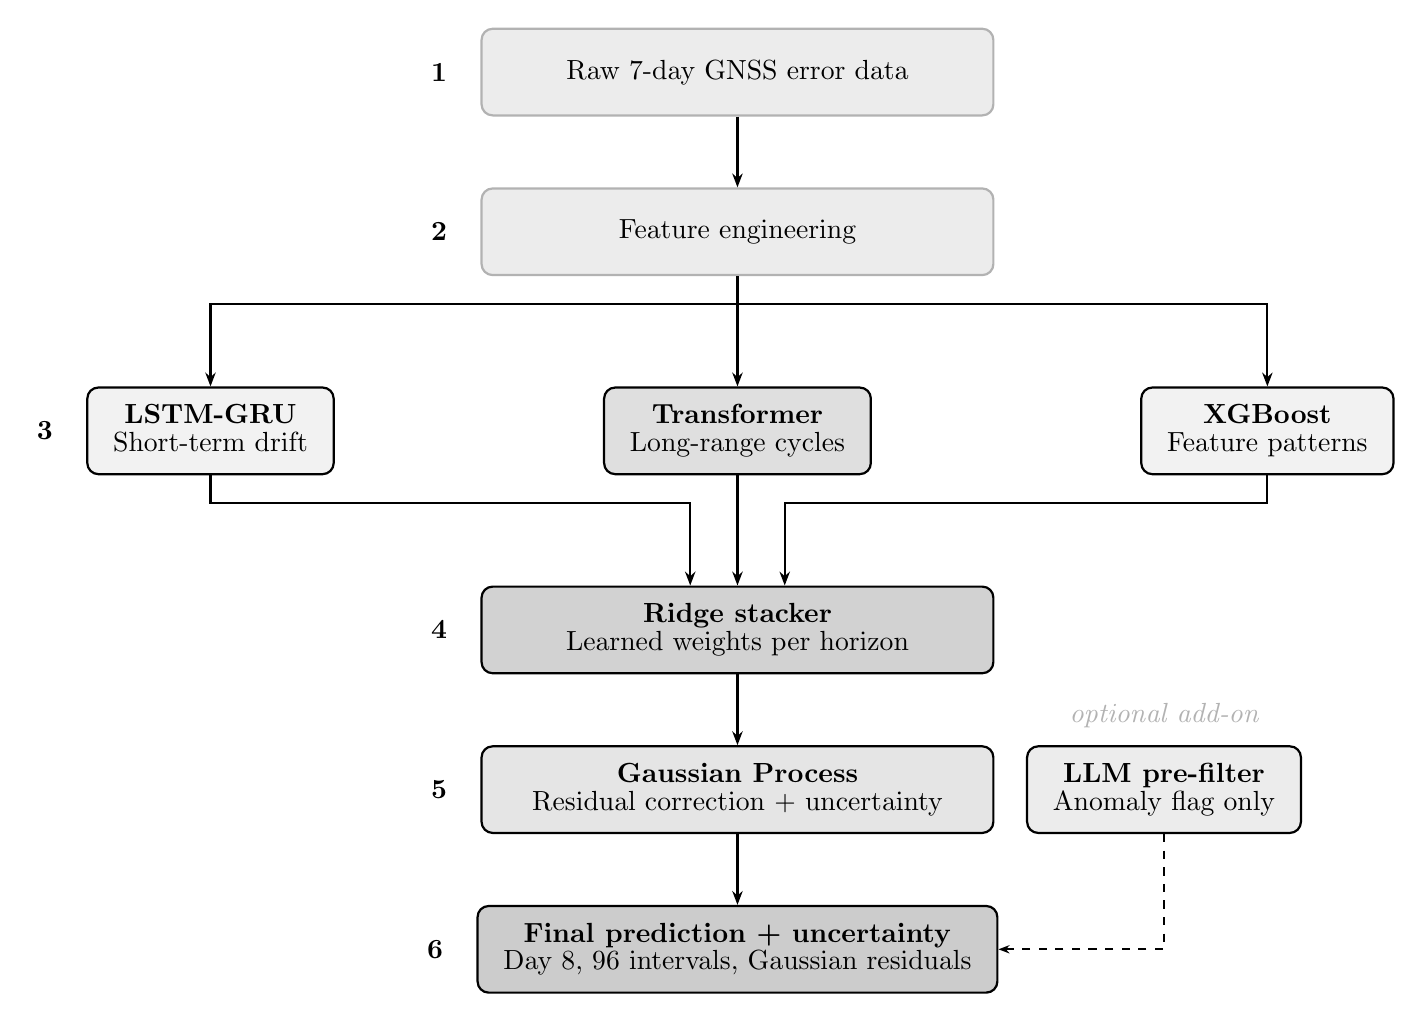
\begin{tikzpicture}[
    node distance = 0.9cm and 0.4cm,
    base/.style = {
        rectangle, rounded corners=4pt,
        minimum height=1.1cm, text centered,
        font=\normalsize, draw, thick
    },
    gray/.style   = {base, fill=gray!15, draw=gray!60,  text=black, minimum width=6.5cm},
    blue/.style   = {base, fill=gray!10, draw=black,    text=black, minimum width=2.8cm},
    purple/.style = {base, fill=gray!25, draw=black,    text=black, minimum width=2.8cm},
    teal/.style   = {base, fill=gray!10, draw=black,    text=black, minimum width=2.8cm},
    amber/.style  = {base, fill=gray!35, draw=black,    text=black, minimum width=6.5cm},
    coral/.style  = {base, fill=gray!20, draw=black,    text=black, minimum width=6.5cm},
    green/.style  = {base, fill=gray!40, draw=black,    text=black, minimum width=6.5cm},
    pink/.style   = {base, fill=gray!15, draw=black,    text=black, minimum width=2.5cm},
    steplabel/.style = {font=\normalsize\bfseries, text=black},
    sublabel/.style  = {font=\normalsize,           text=gray!60!black},
    arr/.style = {-{Stealth[length=5pt]}, thick, black}
]
\node[gray]   (raw)    {Raw 7-day GNSS error data};
\node[steplabel, left=0.3cm of raw] {1};
\node[gray, below=of raw]  (feat)   {Feature engineering};
\node[steplabel, left=0.3cm of feat] {2};
\node[blue,   below left =1.4cm and 1.85cm of feat] (lstm)
    {\begin{tabular}{c}\textbf{LSTM-GRU}\\[-2pt]{\normalsize Short-term drift}\end{tabular}};
\node[purple, below=1.4cm of feat] (trans)
    {\begin{tabular}{c}\textbf{Transformer}\\[-2pt]{\normalsize Long-range cycles}\end{tabular}};
\node[teal,   below right=1.4cm and 1.85cm of feat] (xgb)
    {\begin{tabular}{c}\textbf{XGBoost}\\[-2pt]{\normalsize Feature patterns}\end{tabular}};
\node[steplabel, left=0.3cm of lstm] {3};
\node[amber, below=1.4cm of trans] (stacker)
    {\begin{tabular}{c}\textbf{Ridge stacker}\\[-2pt]{\normalsize Learned weights per horizon}\end{tabular}};
\node[steplabel, left=0.3cm of stacker] {4};
\node[coral, below=of stacker] (gp)
    {\begin{tabular}{c}\textbf{Gaussian Process}\\[-2pt]{\normalsize Residual correction + uncertainty}\end{tabular}};
\node[steplabel, left=0.3cm of gp] {5};
\node[pink, right=0.4cm of gp] (llm)
    {\begin{tabular}{c}\textbf{LLM pre-filter}\\[-2pt]{\normalsize Anomaly flag only}\end{tabular}};
\node[font=\normalsize\itshape, text=gray!60, above=0.1cm of llm] {optional add-on};
\node[green, below=of gp] (out)
    {\begin{tabular}{c}\textbf{Final prediction + uncertainty}\\[-2pt]{\normalsize Day 8, 96 intervals, Gaussian residuals}\end{tabular}};
\node[steplabel, left=0.3cm of out] {6};
\draw[arr] (raw)   -- (feat);
\draw[arr] (feat.south) -- ++(0,-0.35) -| (lstm.north);
\draw[arr] (feat.south) -- (trans.north);
\draw[arr] (feat.south) -- ++(0,-0.35) -| (xgb.north);
\draw[arr] (lstm.south) -- ++(0,-0.35) -| ([xshift=-0.6cm]stacker.north);
\draw[arr] (trans.south) -- (stacker.north);
\draw[arr] (xgb.south)  -- ++(0,-0.35) -| ([xshift=+0.6cm]stacker.north);
\draw[arr] (stacker) -- (gp);
\draw[arr] (gp) -- (out);
\draw[-{Stealth[length=4pt]}, dashed, thick, black]
    (llm.south) -- (llm.south |- out.east) -- (out.east);
\end{tikzpicture}
}%
\caption{Proposed multi-pipeline ensemble architecture for GNSS broadcast error prediction.}
\label{fig:pipeline}
\end{figure}

\subsection{Problem Formulation}\label{AA}

At time $t$, let $e(t)$ denote the deviation between the transmitted value and the true physical value (e.g., clock offset or orbital parameter error). Given a historical sequence of length $L$ (where $L = 96$, corresponding to one day sampled at 15-minute intervals), the objective is to predict the future value $e(t + h)$.

The forecasting horizon $h$ represents the number of steps ahead and takes values from the set $\{1, 2, 4, 8, \dots, 96\}$, corresponding to prediction intervals ranging from 15 minutes to 24 hours. These horizons enable modeling both short-term and long-term temporal dependencies.

The model is trained using data from seven consecutive days, capturing temporal patterns and periodic behaviors. Evaluation is performed on the eighth day, which consists of 96 time steps. This test set is strictly held out and is not used during training. Predictions are generated for this final day and compared against ground truth values to assess model performance.

\subsection{Feature Engineering}

The feature engineering process constructs two complementary representations of the data: one capturing the raw temporal sequence and the other encoding derived statistical and temporal characteristics.

\begin{itemize}

\item \textbf{Sequential Representation:}  
A uni-variate sequence representation, denoted as $X_{\text{seq}}$, contains the raw error values without any transformation. This representation preserves the temporal ordering of the data and is directly provided as input to sequence-based models such as LSTM-GRU and Transformer architectures. By maintaining the original structure, these models can effectively learn temporal dependencies and dynamic patterns present in the data.

\item \textbf{Derived Feature Representation:}  
A set of engineered features is constructed to capture temporal dynamics and statistical properties. Lag features are generated at intervals of $\{1, 2, 4, 8, 96\}$ time steps to incorporate short-term and long-term dependencies. Additionally, rolling statistics such as moving averages, standard deviation (spread), maximum, and minimum values are computed over a recent window of observations.

To encode periodic behavior, cyclic time features are introduced using sinusoidal transformations to represent daily and half-daily patterns. Furthermore, first-order differences (rate of change) and second-order differences (acceleration of change) are included to capture the dynamics of variation. The forecasting horizon $h$ is also incorporated as an input feature, allowing the model to adapt its predictions based on the prediction distance.

\end{itemize}

All features are integrated into a unified learning framework, ensuring that both sequential and engineered representations contribute jointly without separation.

\subsection{Base Model 1: LSTM-GRU Network}

Starting off, a basic version uses LSTM along with GRU parts to track old patterns and spot fresh changes in numbers. It works well even when there is not much info because it keeps what matters from the past without slowing down too much.

Ahead of everything, the LSTM layer handles the input series $\{x_t\}$, keeping vital earlier data alive via controlled adjustments. Because gates manage flow, long-term signals survive while less useful pieces fade slowly. What happens next depends on how each gate opens or closes at every step. Information sticks around only if the system decides it matters enough.

\begin{align}
f_t &= \sigma(W_f x_t + U_f h_{t-1} + b_f) \\
i_t &= \sigma(W_i x_t + U_i h_{t-1} + b_i) \\
\tilde{c}_t &= \tanh(W_c x_t + U_c h_{t-1} + b_c) \\
c_t &= f_t \odot c_{t-1} + i_t \odot \tilde{c}_t \\
o_t &= \sigma(W_o x_t + U_o h_{t-1} + b_o) \\
h_t &= o_t \odot \tanh(c_t)
\end{align}

Inside, memory moves when switches — like $f_t$, $i_t$, $o_t$ — decide what stays, shaped by earlier inputs. Signals slip away unless these gates hold them tight across steps.

From the LSTM, signals move into a GRU section. This part cuts down on complex switches but holds onto time-based patterns just fine.

\begin{align}
z_t &= \sigma(W_z x_t + U_z h_{t-1} + b_z) \\
r_t &= \sigma(W_r x_t + U_r h_{t-1} + b_r) \\
\tilde{h}_t &= \tanh(W_h x_t + U_h (r_t \odot h_{t-1}) + b_h) \\
h_t &= (1 - z_t) \odot h_{t-1} + z_t \odot \tilde{h}_t
\end{align}

A fresh take on the LSTM output comes from the GRU, which shapes it further before sending its last hidden state onward. That state moves into two dense layers, one after another, each transforming the data slightly. Out of this chain emerges just one number, the model's final guess.

Stability during training comes from using the Adam optimizer together with gradient clipping, which keeps large updates under control. Before anything else happens, target values get scaled down — then returned to normal size once testing begins.

A chunk at the end — just fifteen percent of the training data — is held back to check how things are going. When that held-back portion shows no real progress, the system slows down on its own. Improvement pauses there mean learning ends early, which keeps results from sticking too closely to one dataset.

\subsection{Base Model 2: Temporal Transformer}

One step further, a Transformer encoder[14] takes shape — this version uses trained position markers to notice patterns across distant points in time, also catching repeating cycles. Into this setup, the input flows as a sequence, lifted into a $d_{\text{model}}$-sized vector space where location tags join in. 

At every stage, attention heads scan all moment pairs at once, not one after another but altogether. This interaction is defined through scaled dot-product attention:

\begin{align}
\text{Attention}(Q, K, V) = \text{softmax}\left(\frac{QK^T}{\sqrt{d_k}}\right)V
\end{align}

Multiple attention heads work in parallel to capture different relationships:

\begin{align}
\text{MultiHead}(Q, K, V) = \text{Concat}(\text{head}_1, \dots, \text{head}_h)W^O
\end{align}

After that, small networks refine each point separately through a position-wise feed-forward layer:

\begin{align}
\text{FFN}(x) = \max(0, xW_1 + b_1)W_2 + b_2
\end{align}

Because of how it links far-apart timestamps instantly, rhythms lasting up through an entire day-long stretch become easier to grasp. What emerges is a sense for timing that spans the whole cycle without losing thread.

Out at the edge, a small network maps the last token into a prediction. Just like before, training runs the same way the LSTM-GRU setup does — same settings across the board so things line up when we compare[12].

\subsection{Base Model 3: XGBoost}

A different kind of foundation sits with the third option — this one built on boosted trees, specifically XGBoost[14], fed only tabular data called $X_{\text{tab}}$. Unlike neural nets[11], these models thrive when patterns twist and turn within organized inputs, handling messy relationships naturally. They brush off useless columns without fuss, staying reliable even when data amounts stay modest. Little tweaking is needed for solid results, which helps keep things stable.

Here’s a key detail — the forecast distance, labeled $h$, gets tossed directly into the mix as just another column. Because of that, one unified model handles every prediction window at once, letting the branches inside decide how much each factor matters depending on how far ahead it looks.

The model builds predictions through an additive process of decision trees:

\begin{align}
\hat{y}_i = \sum_{k=1}^{K} f_k(x_i), \quad f_k \in \mathcal{F}
\end{align}

where each $f_k$ represents a regression tree and $\mathcal{F}$ is the space of all possible trees.

Training minimizes a regularized objective:

\begin{align}
\mathcal{L} = \sum_{i} l(y_i, \hat{y}_i) + \sum_{k} \Omega(f_k)
\end{align}

where $l(\cdot)$ is the loss function (e.g., squared error) and $\Omega(f_k)$ controls model complexity.

When the validation error begins to rise, training stops. Part of each dataset gets used at every step, along with a fraction of the features. This helps keep predictions from fitting too closely to noise.

\subsection{Ridge Regression Meta-Learner}

One after another, the three starting models deliver forecasts: $p_{\text{LSTM}}$, then $p_{\text{Transformer}}$, followed by $p_{\text{XGB}}$. Instead of adding them directly, a secondary method — Ridge regression — weaves these together. It learns how to blend them using past predictions made during cross-validation rounds.

Those earlier guesses sit inside a structure shaped like $[p_{\text{LSTM}},\; p_{\text{Transformer}},\; p_{\text{XGB}}]$, matched against actual outcomes. Only data held aside for checking — not used when first models were built — feeds into this step. By working solely with untouched cases, the blending rule cannot favor a model that merely memorized its lessons too closely. What emerges instead reflects which one actually handles new situations best.

The Ridge regression model combines predictions through a linear mapping:

\begin{align}
\hat{y}_h = w_1 p_{\text{LSTM}} + w_2 p_{\text{Transformer}} + w_3 p_{\text{XGB}} + b
\end{align}

where $w_1, w_2, w_3$ are learned weights and $b$ is a bias term.

Training minimizes a regularized objective:

\begin{align}
\mathcal{L} = \sum_{i} (y_i - \hat{y}_i)^2 + \lambda \sum_{j} w_j^2
\end{align}

which keeps the weights from growing too large while fitting the data.

One unique meta-learner handles each forecast window, shaping weights tailored to that timeframe. Because of this setup, it might decide the Transformer matters more when looking 24 hours ahead — orbital cycles play a bigger role then. In contrast, for predictions just 15 minutes out, patterns in immediate past data become key, favoring the LSTM-GRU blend[12]. Each combined output ends up labeled as $\hat{y}_h$.

\subsection{Gaussian Process Residual Model}

With each model missing some patterns, what’s left — like shifting trends or repeating cycles — sticks around in the leftover signal $r_h$. Instead of vanishing, these bits get caught by a flexible smoother built on probability rules. That extra layer adjusts the main forecast slightly while also sketching how unsure it feels about that fix.

The residual is defined as:
\begin{align}
r_h = y_h - \hat{y}_h
\end{align}

Apart from the Matérn part, the GP uses a mix of kernels — specifically $k_{\text{Matérn}}$ joined with $k_{\text{Periodic}}$ — to handle different patterns:

\begin{align}
k(x, x') = k_{\text{Matérn}}(x, x') + k_{\text{Periodic}}(x, x')
\end{align}

While one piece models rough but continuous leftovers, another picks up repeating signals tied to orbit timing. Instead of fixed settings, values for these parts adjust by maximizing the log marginal likelihood of observed data:

\begin{align}
\log p(\mathbf{y} \mid X) = -\frac{1}{2} \mathbf{y}^T K^{-1} \mathbf{y} - \frac{1}{2} \log |K| - \frac{n}{2} \log 2\pi
\end{align}

When making estimates, average outcomes come from updated beliefs, whereas spread across possible results shows prediction confidence. The Gaussian Process produces:

\begin{align}
\mu_{\text{GP}}(x_*) &= K_*^T K^{-1} \mathbf{y} \\
\sigma^2_{\text{GP}}(x_*) &= K(x_*, x_*) - K_*^T K^{-1} K_*
\end{align}

At time $t + h$, the estimate lines up with $\hat{y}_h$ combined with $\mu_{\text{GP}}$ instead:

\begin{align}
\hat{y}_h^{\text{final}} = \hat{y}_h + \mu_{\text{GP}}
\end{align}

Spread at that point matches $\sigma_{\text{GP}}$ from the model output directly.

Most of the time, leftover errors after using group predictions look random. That happens because how we build the model makes those leftovers follow a bell-shaped pattern. If the main set of models handles the biggest mistakes well, what remains acts like steady, unconnected noise. So, future forecast differences — what actually happens minus what was predicted — tend to spread out in a way that matches normal curves fairly closely. Meeting this shape check means the gaps behave much like standard statistical noise should.

\subsection{Summary of Architecture}
\begin{table}[H]
\caption{Summary of Proposed Ensemble Components}
\begin{center}
\resizebox{\columnwidth}{!}{%
\begin{tabular}{|c|c|c|c|}
\hline
\textbf{Component} & \textbf{Role} & \textbf{Input} & \textbf{Strength} \\
\hline
LSTM-GRU & Short-term dynamics & Raw sequence (96$\times$1) & Sequential memory, drift capture \\
\hline
Transformer & Long-range periodicity & Raw sequence (96$\times$1) & Orbital cycle, global attention \\
\hline
XGBoost & Feature-based patterns & Lag, rolling, sin/cos & Nonlinear tabular relationships \\
\hline
Ridge stacker & Optimal blending & 3 model predictions & Per-horizon learned weights \\
\hline
Gaussian Process & Residual + uncertainty & Stacker residuals & Gaussian output, uncertainty \\
\hline
\end{tabular}}
\label{tab:architecture}
\end{center}
\end{table}

\section{Conclusion}
One way to look at it starts with stacking different models together - LSTM-GRU, Transformer, plus XGBoost - not simply added but woven through a Ridge method that shifts based on time ahead. Instead of treating predictions as fixed numbers, randomness gets shaped into usable ranges using Gaussian Processes so results feel more trustworthy when checking system safety. While each part does its job separately, their joint behavior shows promise especially over varying forecast lengths. What happens next likely involves testing every span head-to-head versus simpler versions just to see where gaps open up. Not everything proves itself right away though some clues point forward anyway.

\section*{Acknowledgment}

This work was carried out independently, without any external funding or institutional support. We are grateful to ISRO, the organizers of the GNSS error prediction challenge for making the dataset available and for posing a problem that genuinely pushed us to think carefully about the structure of satellite errors. We also thank the developers of PyTorch, XGBoost, and GPyTorch. Without these tools, none of this would have been practical to build.

\begin{thebibliography}{16}

\bibitem{1}
IGS, ``International GNSS Service: Products,'' \textit{igs.org}, 2024.

\bibitem{2}
IS-GPS-200, ``Navstar GPS Space Segment/Navigation User Interfaces,'' Interface Specification, Rev. N, 2022.

\bibitem{3}
O.~Montenbruck \textit{et al.}, ``Precise orbit determination of GNSS satellites,'' in \textit{Springer Handbook of Global Navigation Satellite Systems}, 2017.

\bibitem{4}
Y.~Wang \textit{et al.}, ``Satellite clock bias prediction based on support vector regression,'' \textit{GPS Solutions}, vol.~21, 2017.

\bibitem{5}
G.~Huang \textit{et al.}, ``Neural network-based GNSS clock prediction,'' \textit{Advances in Space Research}, vol.~63, 2019.

\bibitem{6}
X.~Li \textit{et al.}, ``LSTM-based satellite clock bias prediction,'' \textit{IEEE Access}, vol.~8, 2020.

\bibitem{7}
J.~Guo \textit{et al.}, ``Deep learning for GPS satellite clock error prediction,'' \textit{Remote Sensing}, vol.~13, 2021.

\bibitem{8}
A.~Vaswani \textit{et al.}, ``Attention is all you need,'' in \textit{NeurIPS}, 2017.

\bibitem{9}
C.~E.~Rasmussen and C.~K.~I.~Williams, \textit{Gaussian Processes for Machine Learning}, MIT Press, 2006.

\bibitem{10}
S.~Makridakis \textit{et al.}, ``The M4 competition: Results, findings, conclusion and way forward,'' \textit{International Journal of Forecasting}, vol.~34, 2018.

\bibitem{11}
D.~Wolpert, ``Stacked generalization,'' \textit{Neural Networks}, vol.~5, 1992.

\bibitem{12}
S.~Hochreiter and J.~Schmidhuber, ``Long short-term memory,'' \textit{Neural Computation}, vol.~9, 1997.

\bibitem{13}
K.~Cho \textit{et al.}, ``Learning phrase representations using RNN encoder-decoder,'' in \textit{EMNLP}, 2014.

\bibitem{14}
T.~Chen and C.~Guestrin, ``XGBoost: A scalable tree boosting system,'' in \textit{KDD}, 2016.

\end{thebibliography}

\vspace{12pt}

\end{document}